%%%%%%%%%%%%%%%%%%%%%%%%%%%%%%%%%%%%%%%%%%%%%%%%%%%%%%%
%%%%% Sec: Differentiable programming %%%%%
%%%%%%%%%%%%%%%%%%%%%%%%%%%%%%%%%%%%%%%%%%%%%%%%%%%%%%%
\section{Differentiable programming}
\label{sec:diff_prog}

Differentiable programming is an advanced computational paradigm that unites traditional programming concepts with the principles of differentiation, a fundamental concept in calculus. This approach extends the idea of computing derivatives to entire programs, enabling the automatic calculation of gradients of program outputs with respect to inputs. Differentiable programming is particularly powerful in the context of optimization, machine learning, and artificial intelligence, where it facilitates efficient parameter tuning to minimize or maximize some objective function.
Methods for computing derivatives in computer programs can be classified into four categories (see \cref{fig:diff_methods}):
\begin{enumerate}
    \item manually working out derivatives and coding them;
    \item \textbf{numerical differentiation}, involves approximating the derivative of a function using values of the original function evaluated at some sample points \citep{burden_numerical_2016}. In its simplest form, it is based on the limit definition of a derivative. It is quite simple to implement and apply to a wide range of problems, especially when dealing with data-driven models or functions that lack a clear analytical representation. Its effectiveness diminishes in high-dimensional settings, where the complexity and computational demands increase exponentially, highlighting the method's limitations in handling complex, multi-variable functions efficiently;
    \item \textbf{symbolic differentiation}, which refers to the automatic process of finding derivatives using the rules of differentiation to obtain an exact symbolic expression for the derivative of a given function \citep{grabmeier_computer_2003}. This method works similarly to how humans perform differentiation ``by hand'', manipulating symbols according to mathematical laws;
    \item \textbf{automatic differentiation} (AD), also called algorithmic differentiation,is a method that computes the derivative of a function efficiently and accurately by systematically applying the chain rule of calculus to the sequence of elementary operations (additions, multiplications, trigonometric functions, etc.) that constitute a computer program. All numerical computations are ultimately compositions of a finite set of elementary operations for which derivatives are known \citep{verma_introduction_2000,griewank_evaluating_2008}, and combining the derivatives of the constituent operations through the chain rule of calculus\footnote{The derivative of the composition of two (or more) differentiable functions $f$ and $g$ can be expressed in terms of the derivatives of the single functions $f$ and $g$. If $h (x) = f(g(x))$, then $h^\prime(x) = f^\prime(g(x)) g^\prime(x)$.} gives the derivative of the overall composition. AD is not an approximation like numerical differentiation, but rather computes derivatives to machine precision.
\end{enumerate}
\newpage
In particular, differentiable programming refers to using automatic differentiation in some way that allows a program to optimize its parameters to improve on some task. It only has three requirements:
\begin{enumerate}
    \item a parameterized function/model to be optimized;
    \item (automatic) differentiability of the object to be optimized;
    \item a function suitable to measure the performance of the model.
\end{enumerate}

The process of optimizing a model in the field of differentiable programming is often called \emph{training}.
In the subsequent portion of this section, a comprehensive overview of automatic differentiation and its role in the training process will be provided. This will be followed by an in-depth exposition of the process itself.

\begin{figure}
    \centering
    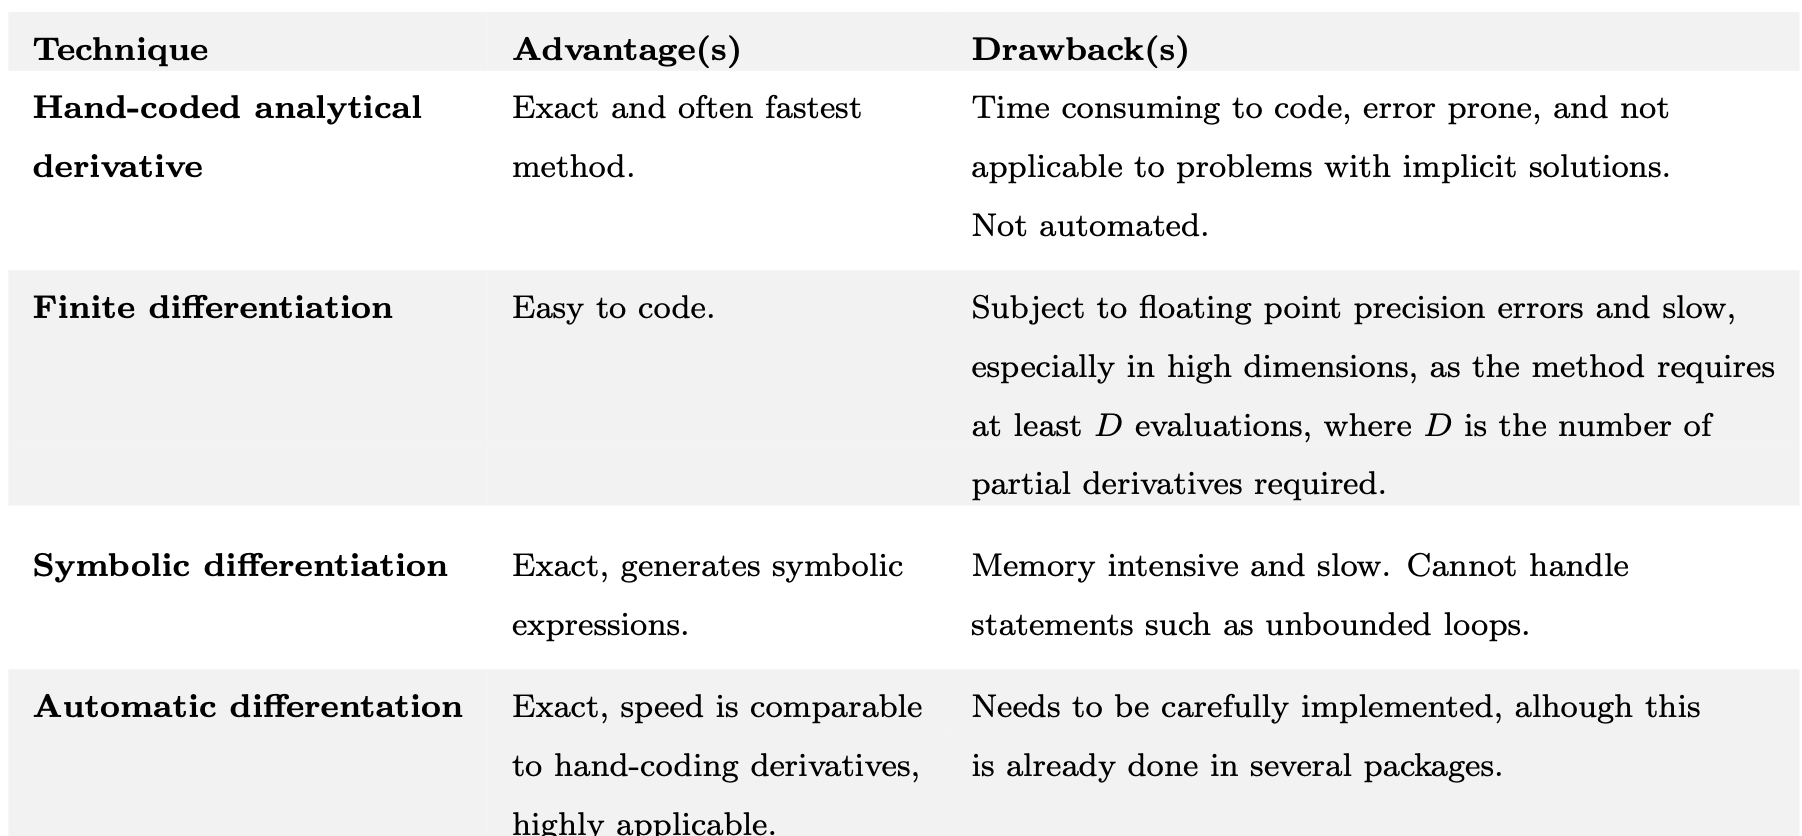
\includegraphics[width=\linewidth, keepaspectratio]{img//chapter4/diff_methods.png}
    \caption[Summary of techniques to calculate derivatives]{Summary of techniques to calculate derivatives.\\\small{Credits: \cite{margossian_review_2019}.}}
    \label{fig:diff_methods}
\end{figure}


%%%%%%%%%%%%%%%%%%%%%%%%%%%%%%%%%%%%%%%%%%%%%%%%%%%%%%%
%%%%% SubSec: Automatic differentiation %%%%%
%%%%%%%%%%%%%%%%%%%%%%%%%%%%%%%%%%%%%%%%%%%%%%%%%%%%%%%
\subsection{Automatic differentiation}
\label{subsec:automatic_differentiation}


%%%%%%%%%%%%%%%%%%%%%%%%%%%%%%%%%%%%%%%%%%%%%%%%%%%%%%%
%%%%% SubSubSec: Computational graph %%%%%
%%%%%%%%%%%%%%%%%%%%%%%%%%%%%%%%%%%%%%%%%%%%%%%%%%%%%%%
\subsubsection{Computational graph}
\label{subsubsec:computational_graph}
As already stated, automatic differentiation operates on the fundamental principle that complex functions can be decomposed into a series of elementary arithmetic operations. Given a target composite function $f (x) = h \circ g(x) = h(g(x))$, with $x \in \mathbb{R}^n$, $g : \mathbb{R}^n \rightarrow \mathbb{R}^k$, and $h : \mathbb{R}^k \rightarrow \mathbb{R}^m$, applying the chain rule and elementary matrix multiplication, the corresponding Jacobian matrix\footnote{The Jacobian matrix of a vector-valued function of several variables is the matrix of all its first-order partial derivatives.} $J$ is thus:
\be
\label{eq:4.1}
J = J_{h \circ g} = J_h (g(x)) \cdot J_g (x) \,,
\ee
with $(i,j)^{th}$ element:
\be
\label{eq:4.2}
J_{ij} = \frac{\partial f_i}{\partial x_j} = \frac{\partial h_i}{\partial g_1} \frac{\partial g_1}{\partial x_j} + \frac{\partial h_i}{\partial g_2} \frac{\partial g_2}{\partial x_j} + \ldots + \frac{\partial h_i}{\partial g_k} \frac{\partial g_k}{\partial x_j} \,.
\ee

More generally, if $f$ is the composite expression of $L$ functions
\be
\label{eq:4.3}
f = f^L \circ f^{L-1} \circ \ldots \circ f^1 \,,
\ee
the corresponding Jacobian matrix will be
\be
\label{eq:4.4}
J = J_L \cdot J_{L-1} \cdot \ldots \cdot J_1 \,.
\ee
Hence, given a complex function $f$, it is possible to break down the action of the Jacobian matrix on a vector into simple components.
So, following \cite{griewank_evaluating_2008} notation, a function $f : \mathbb{R}^n \rightarrow \mathbb{R}^m$ can be constructed using intermediate variables $v_i$ such that
\begin{itemize}
    \item variables $v_{i-n} = x_i$, $i = 1, \ldots, n$ are the input variables,
    \item variables $v_{i}$, $i = 1, \ldots, l$ are the intermediate variables,
    \item variables $y_{m-i} = v_{l-i}$, $i = m-1, \ldots, 0$ are the output variables.
\end{itemize}
The representation of all the elementary operations that take place to construct a certain function $f$ is called the \emph{evaluation trace}, which can also be pictured as a \emph{computational graph} \citep{bauer_computational_1974}, useful for visualizing the dependency relations between intermediate variables. \Cref{fig:computational_graph} shows the computation graph for an example function $f : \mathbb{R}^2 \rightarrow \mathbb{R}$: 
\be
\label{eq:4.5}
f(x_1, x_2) = \ln{(x_1)} + x_1 x_2 - \sin{(x_2)} \,.
\ee

\begin{figure}
    \centering
    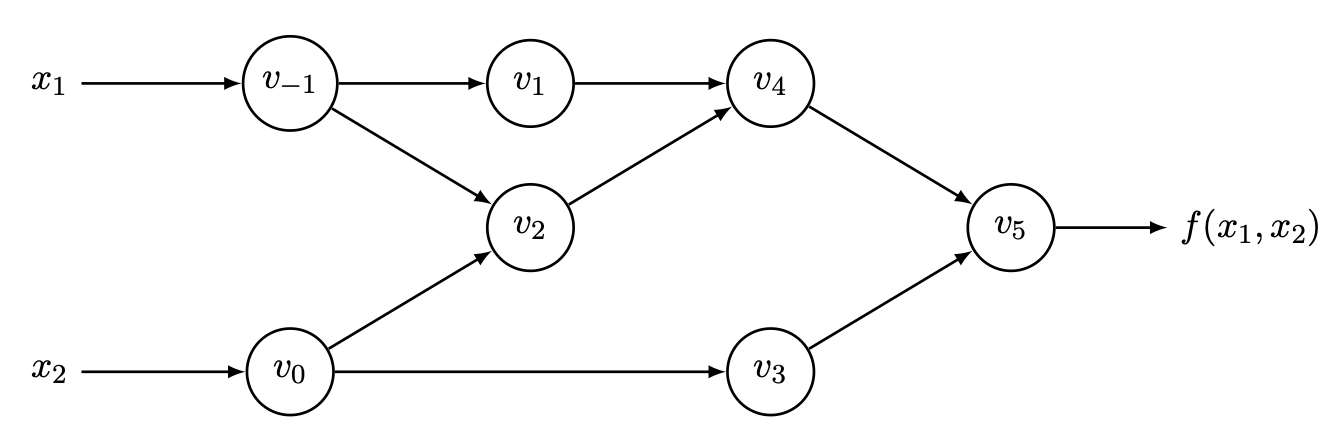
\includegraphics[width=0.9\linewidth, keepaspectratio]{img//chapter4/computational_graph.png}
    \caption[Example of computational graph]{Computational graph of the example $f(x_1, x_2) = \ln{(x_1)} + x_1 x_2 - \sin{(x_2)}$.\\\small{Credits: \cite{baydin_automatic_2018}.}}
    \label{fig:computational_graph}
\end{figure}

Given the computational graph of all elementary operations, AD can be implemented in two main modes: \emph{forward} accumulation mode and \emph{reverse} accumulation mode (backward mode).


%%%%%%%%%%%%%%%%%%%%%%%%%%%%%%%%%%%%%%%%%%%%%%%%%%%%%%%
%%%%% SubSubSec: Forward mode %%%%%
%%%%%%%%%%%%%%%%%%%%%%%%%%%%%%%%%%%%%%%%%%%%%%%%%%%%%%%
\subsubsection{Forward mode}
\label{subsubsec:forward_mode}
Automatic differentiation in forward accumulation mode (or \emph{tangent linear} mode) is the conceptually most simple type. The differentiation process is aligned with the function evaluation itself. Starting from the inputs, the program computes both the function's value and its derivative step by step through the computation graph. For each elementary operation, the forward mode calculates the derivative of the output with respect to the inputs, carrying these derivatives (or ``tangents'') forward through the computation graph.

Considering as an example the evaluation trace of the function defined in \cref{eq:4.5} (left-hand side of \cref{fig:forward_trace}), for computing the derivative of $f$ with respect to $x_1$, the first step is to associate with each intermediate variable $v_i$ a derivative
\be
\label{eq:4.6}
\Dot{v}_i = \frac{\partial v_i}{\partial x_1}.
\ee

Applying then the chain rule to each elementary operation in the forward primal trace, the corresponding tangent (derivative) trace is generated (right-hand side of \cref{fig:forward_trace}), until the required derivative in the final variable $\Dot{v}_5 = \frac{\partial y}{\partial x_1}$ is obtained.

Generalizing this procedure to a function $f : \mathbb{R}^n \rightarrow \mathbb{R}^m$, each forward pass of AD provides one column of the Jacobian matrix (\ie the partial derivatives of all output variables with respect to one input variable).
Thus, the complete Jacobian can be computed in $n$ evaluations. For this reason, forward AD is efficient and straightforward especially for functions $f : \mathbb{R} \rightarrow \mathbb{R}^m$, for which all derivatives can be computed with just one forward pass.

In general, for functions with many inputs $f : \mathbb{R}^n \rightarrow \mathbb{R}^m$ where $n \gg m$, the reverse accumulation mode of AD is preferred.

\begin{figure}
    \centering
    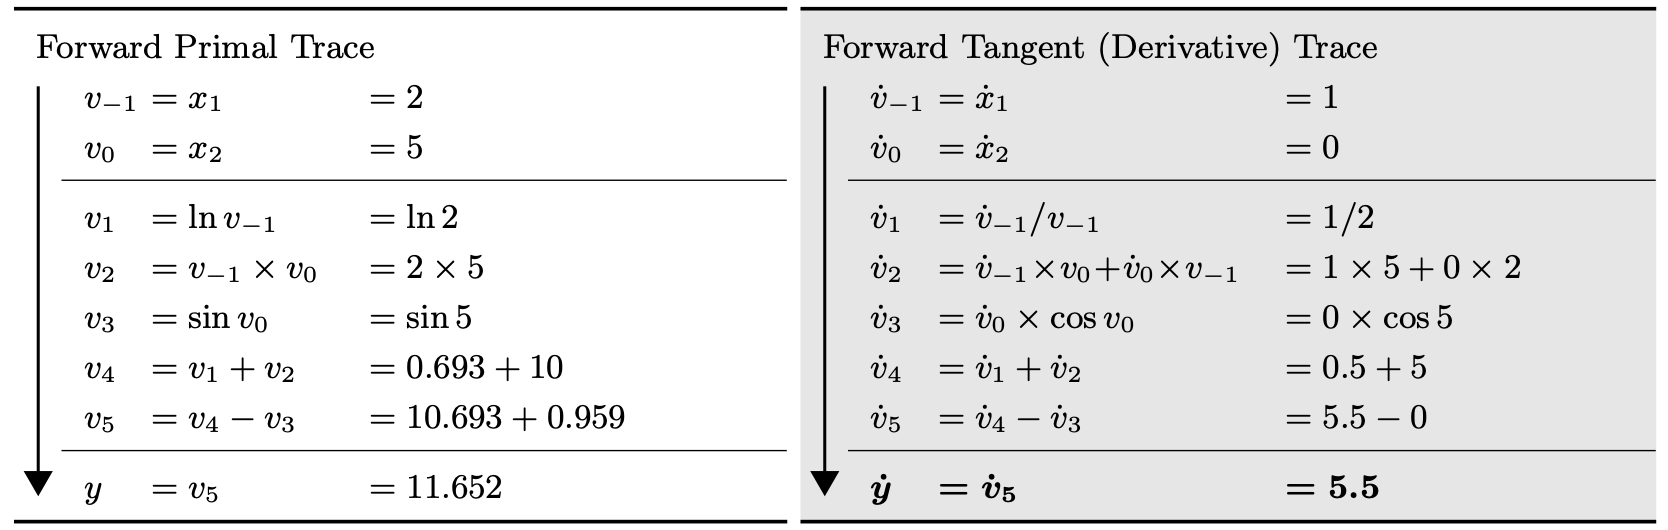
\includegraphics[width=\linewidth]{img//chapter4/forward_trace.png}
    \caption[Forward mode AD example]{Forward mode AD example for $f(x_1, x_2) = \ln{(x_1)} + x_1 x_2 - \sin{(x_2)}$, evaluated at $(x_1, x_2) = (2, 5)$ by setting $\Dot{x}_1 = 1$. The original forward evaluation of the primals on the left is augmented by the tangent operations on the right, where each line complements the original directly to its left.\\\small{Credits: \cite{baydin_automatic_2018}.}}
    \label{fig:forward_trace}
\end{figure}


%%%%%%%%%%%%%%%%%%%%%%%%%%%%%%%%%%%%%%%%%%%%%%%%%%%%%%%
%%%%% SubSubSec: Reverse mode %%%%%
%%%%%%%%%%%%%%%%%%%%%%%%%%%%%%%%%%%%%%%%%%%%%%%%%%%%%%%
\subsubsection{Reverse mode}
\label{subsubsec:reverse_mode}
AD in reverse accumulation mode (or \emph{adjoint} or \emph{cotangent linear} mode) \citep{griewank_numerical_2012} corresponds to a generalized backpropagation algorithm, in that it propagates derivatives backward from a given output. This is done by complementing each variable $v_i$ with an adjoint
\be
\label{eq:4.7}
\overline{v}_i = \frac{\partial y_j}{\partial v_i} \,,
\ee
which represents the sensitivity of a considered output $y_j$ with respect to changes in $v_i$.

In reverse mode AD, derivatives are computed in the second of a two-phase process. In the first phase, the original function code is run forward, creating intermediate variables $v_i$ and recording the dependencies in the computational graph. In the second phase, derivatives are calculated by propagating adjoints $\overline{v}_i$ in reverse, from outputs to inputs. The reverse mode AD for the example function of \cref{eq:4.5} is shown in \cref{fig:reverse_trace}.

An important advantage of the reverse mode is that it is significantly less costly to evaluate (in terms of operation count) than the forward mode for functions with a large number of inputs. In the extreme case of $f : \mathbb{R}^n \rightarrow \mathbb{R}$, only one application of the reverse
mode is sufficient to compute the full gradient, compared with the $n$ passes of the forward mode needed to populate the same. Because the optimization of astrophysical and gravitational lensing parametric functions usually involves the gradient of a scalar-valued objective with respect to a (large) number of parameters, this establishes the reverse mode, as opposed to the forward mode, as the mainstay technique in the form of the backpropagation algorithm \citep{schmidhuber_deep_2015}.

\begin{figure}
    \centering
    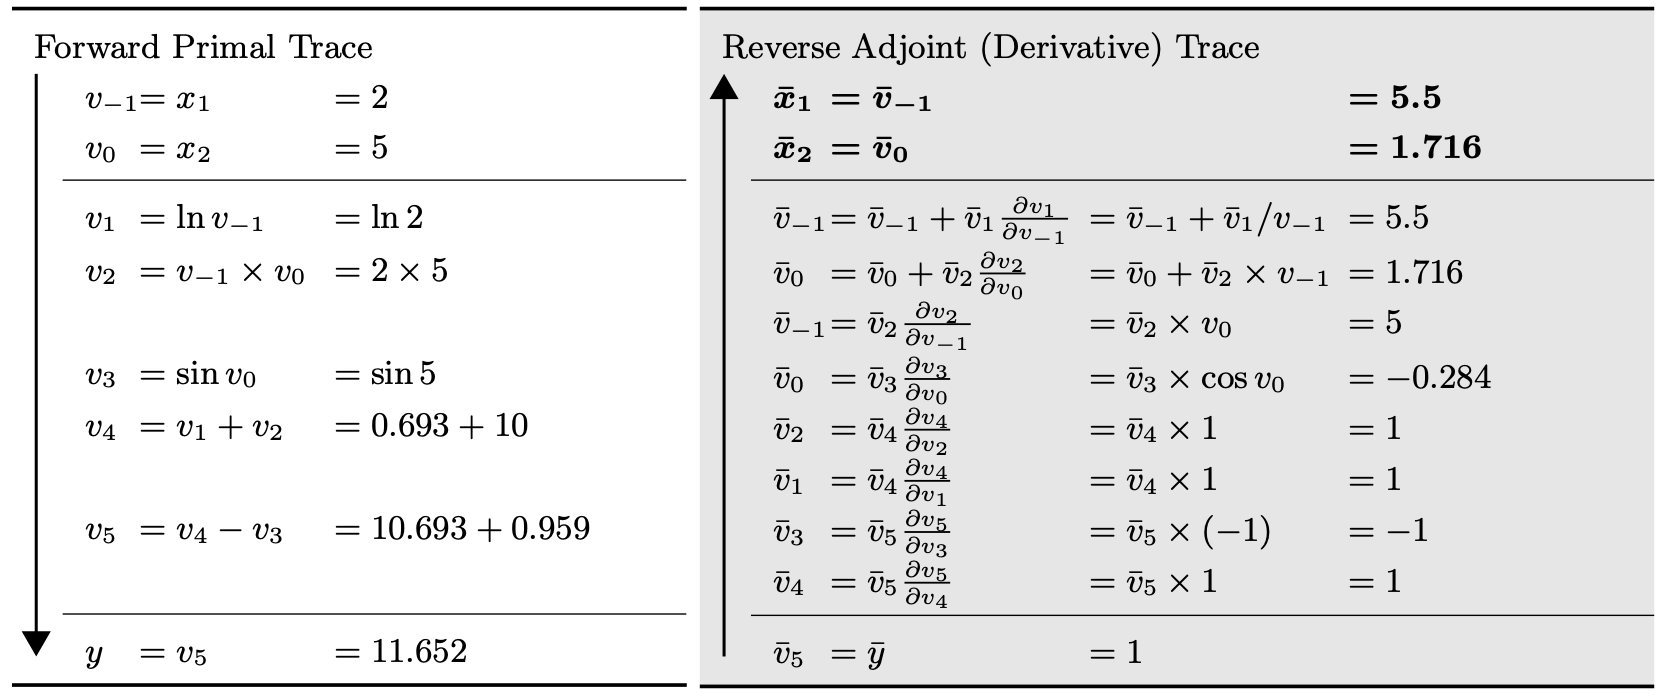
\includegraphics[width=0.9\linewidth, keepaspectratio]{img//chapter4/reverse_trace.png}
    \caption[Reverse mode AD example]{Reverse mode AD example for $f(x_1, x_2) = \ln{(x_1)} + x_1 x_2 - \sin{(x_2)}$, evaluated at $(x_1, x_2) = (2, 5)$. After forward evaluation of the primals on the left, adjoint operations on the right are evaluated in reverse.\\\small{Credits: \cite{baydin_automatic_2018}.}}
    \label{fig:reverse_trace}
\end{figure}


%%%%%%%%%%%%%%%%%%%%%%%%%%%%%%%%%%%%%%%%%%%%%%%%%%%%%%%
%%%%% SubSec: Backpropagation algorithm %%%%%
%%%%%%%%%%%%%%%%%%%%%%%%%%%%%%%%%%%%%%%%%%%%%%%%%%%%%%%
\subsection{Backpropagation algorithm}
\label{subsec:backpropagation_algorithm}
The backpropagation algorithm is the cornerstone of neural network training \citep{rumelhart_learning_1986,montavon_efficient_2012}, mainly used to minimize the error by adjusting the weights of the connections in the network. However, when it comes to a model optimization problem outside the realm of neural networks, such as training parametric models, the concept of backpropagation refers to the method of computing gradients efficiently using reverse mode AD.

The training process (or better, the training loop) is characterized by a sequence of operations performed recursively. The optimization itself is performed by an \emph{optimizer} which operates by tweaking the model parameters in a certain way, with the purpose of minimizing a \emph{loss} function, which quantifies the difference between the predicted outputs of the model and the actual target/observed values. 
The main algorithm that allows for this optimization is the so-called \emph{gradient descent.}


%%%%%%%%%%%%%%%%%%%%%%%%%%%%%%%%%%%%%%%%%%%%%%%%%%%%%%%
%%%%% SubSubSec: Loss function %%%%%
%%%%%%%%%%%%%%%%%%%%%%%%%%%%%%%%%%%%%%%%%%%%%%%%%%%%%%%
\subsubsection{Loss function}
\label{subsubsec:loss_func}
As mentioned above, the loss function provides a measure of the performance of the model. The goal of optimization is to adjust the model parameters in a way that minimizes the loss function. The choice of loss function depends on the specific problem and the model.
Common examples include the Mean Squared Error (MSE) for regression problems
\be
\label{eq:4.8}
\mathrm{MSE} = \frac{1}{n} \sum_{i=1}^n (y_i - \hat{y}_i)^2 \,,
\ee
where $y_i$ and $\hat{y_i}$ are the observed and predicted values, respectively, and the Cross-Entropy Loss for classification problems. 

A common loss function used in the optimization of the gravitational lensing models is the chi-squared ($\chi^2$) statistic, which is the sum of squared differences between observed ($y$) and model-predicted ($\hat{y}$) values, normalized by uncertainties ($\s$) in observations:
\be
\label{eq:4.9}
\chi^2 = \sum_{i=1}^n \bp{\frac{y_i - \hat{y}_i}{\s_i}}^2 \,.
\ee

The loss function is a crucial component because it guides the training process by indicating the direction in which the model parameters should be adjusted. 


%%%%%%%%%%%%%%%%%%%%%%%%%%%%%%%%%%%%%%%%%%%%%%%%%%%%%%%
%%%%% SubSubSec: Gradient descent %%%%%
%%%%%%%%%%%%%%%%%%%%%%%%%%%%%%%%%%%%%%%%%%%%%%%%%%%%%%%
\subsubsection{Gradient descent}
\label{subsubsec:grad_descent}
Gradient-based optimization is one of the pillars of machine learning \citep{bottou_optimization_2018} and is one of the most common optimization algorithms for parametric functions. It is used to find the values of the parameters of a function that decrease the loss function as much as possible \citep{chandra_gradient_2022,ruder_overview_2016}. Given a loss function $f : \mathbb{R}^n \rightarrow \mathbb {R}$, and starting from random initial values of the parameters $\vec{\t}$, classical gradient descent has the objective of finding (local) minima
\be
\label{eq:4.10}
\hat{\vec{\t}} = \argmin_{\vec{\t}} f(\vec{\t}) \,,
\ee
which means finding the set of parameters $\hat{\vec{\t}} \in \mathbb{R}^n$ that minimizes the loss function, as shown in \cref{fig:grad_descent}. In complex models, $f$ might have multiple local minima, and the algorithm seeks to find at least one of these, via updates of the form
\be
\label{eq:4.11}
\D \vec{\t} = - \eta \va{\nabla}_{\va{\t}} f
\ee
where $\eta > 0$ is the so-called step size, also known as \emph{learning rate}, which determines how big a step is taken in the direction opposite to the gradient. Choosing the appropriate $\eta$ is crucial; too small, and the algorithm converges slowly, too large, and it can overshoot the minimum or diverge (see \cref{fig:lr_small_high}). Gradient-based methods make use of the fact that $f$ decreases the steepest moving in the direction of the negative gradient. The convergence rate of gradient-based methods is generally improved by adaptive step size techniques that adjust step size $\eta$ on each iteration \citep{duchi_adaptive_2011,schaul_no_2013,kingma_adam_2017}.

\begin{figure}
  \centering
  \subfloat[]{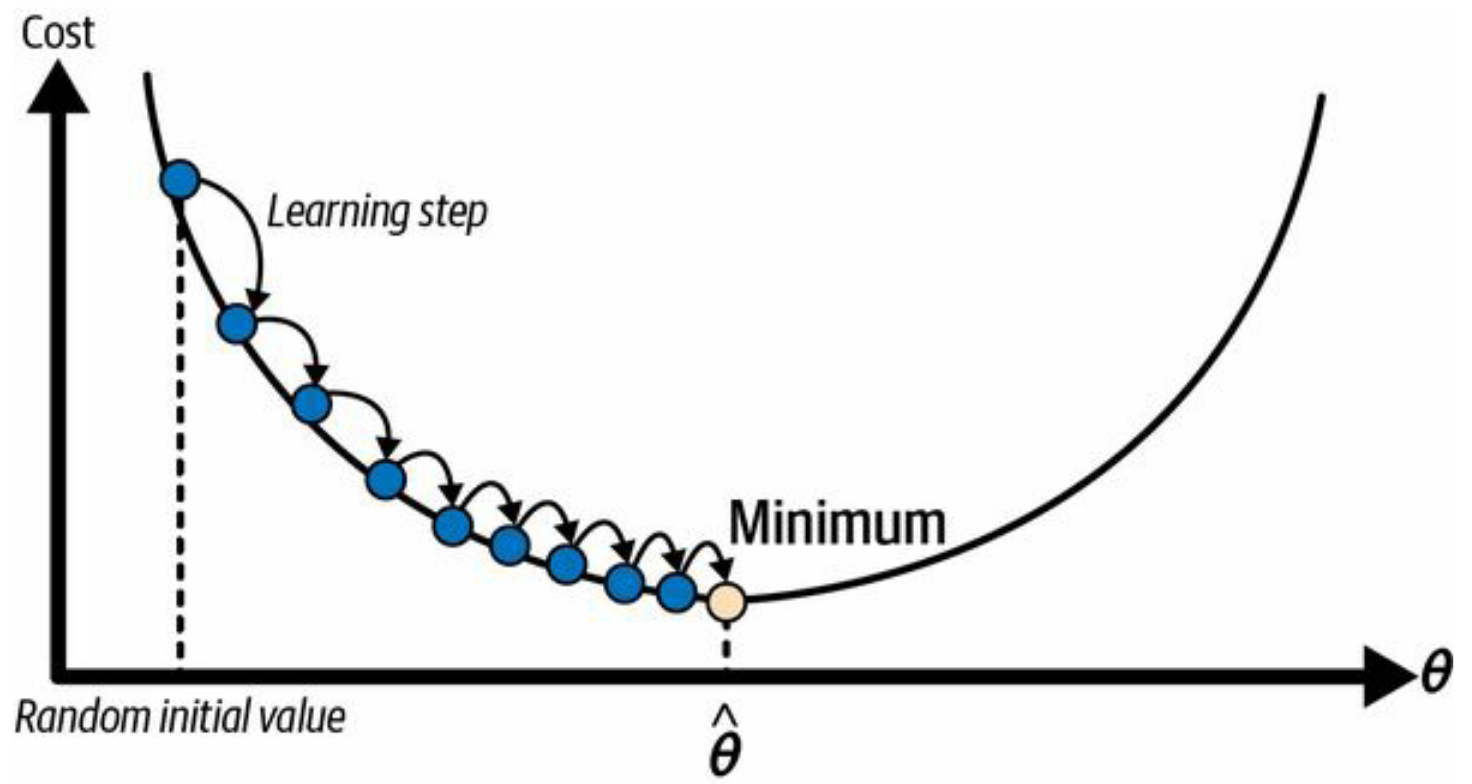
\includegraphics[width=0.5\linewidth, keepaspectratio]{img//chapter4/gradient_descent.png}\label{fig:grad_descent1d}}
  \hfill
  \subfloat[]{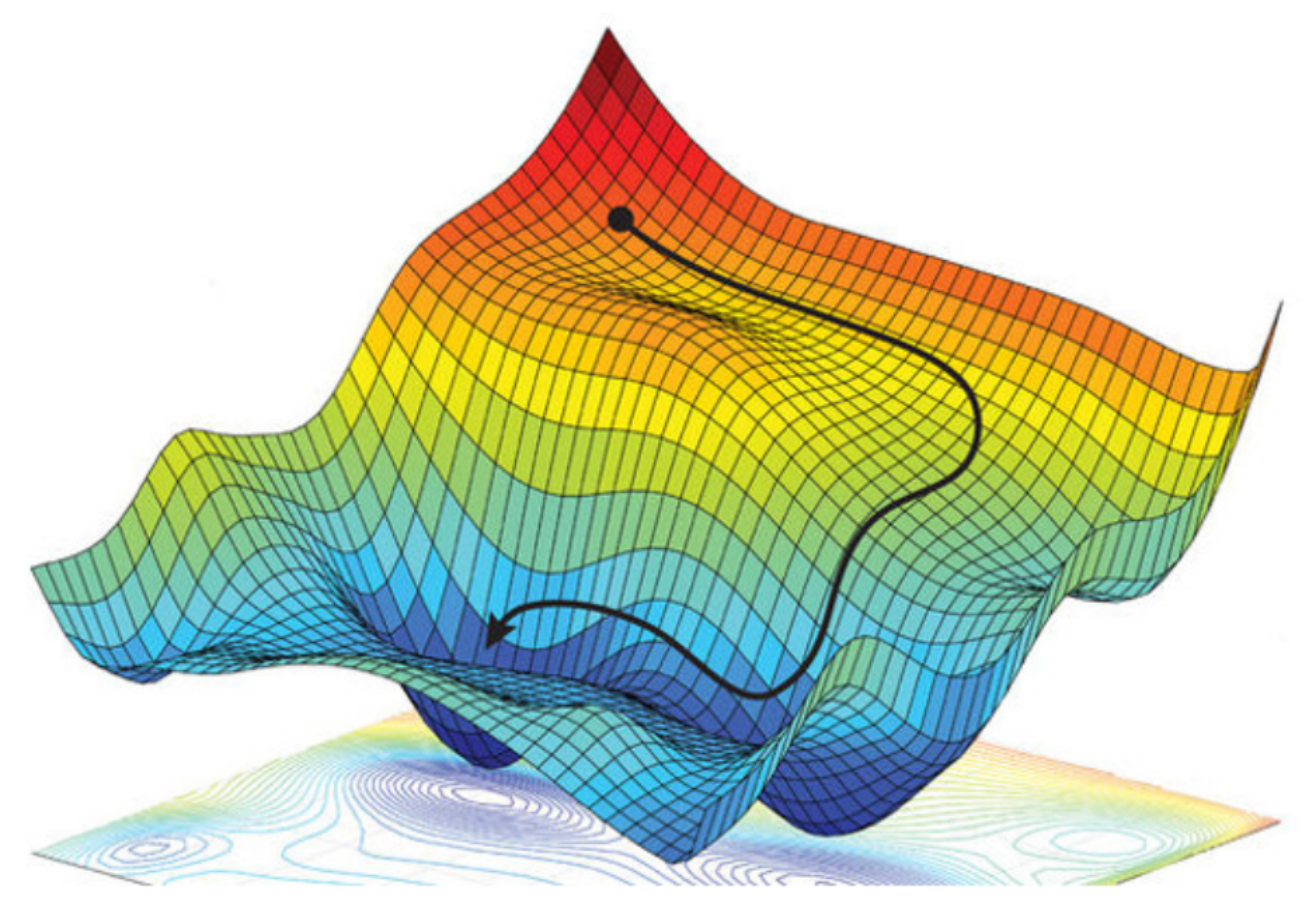
\includegraphics[width=0.5\linewidth, keepaspectratio]{img//chapter4/gradient_descent2d.png}\label{fig:grad_descent2d}}
  \caption[One/two-dimensional gradient descents]{Examples of gradient descents for a \protect\subref{fig:grad_descent1d} one-dimensional loss function and for a \protect\subref{fig:grad_descent2d} two-dimensional one.\\\small{Credits: \cite{geron_hands-machine_2019,amini_spatial_2018}.}}
  \label{fig:grad_descent}
\end{figure}

\begin{figure}
  \centering
  \subfloat[]{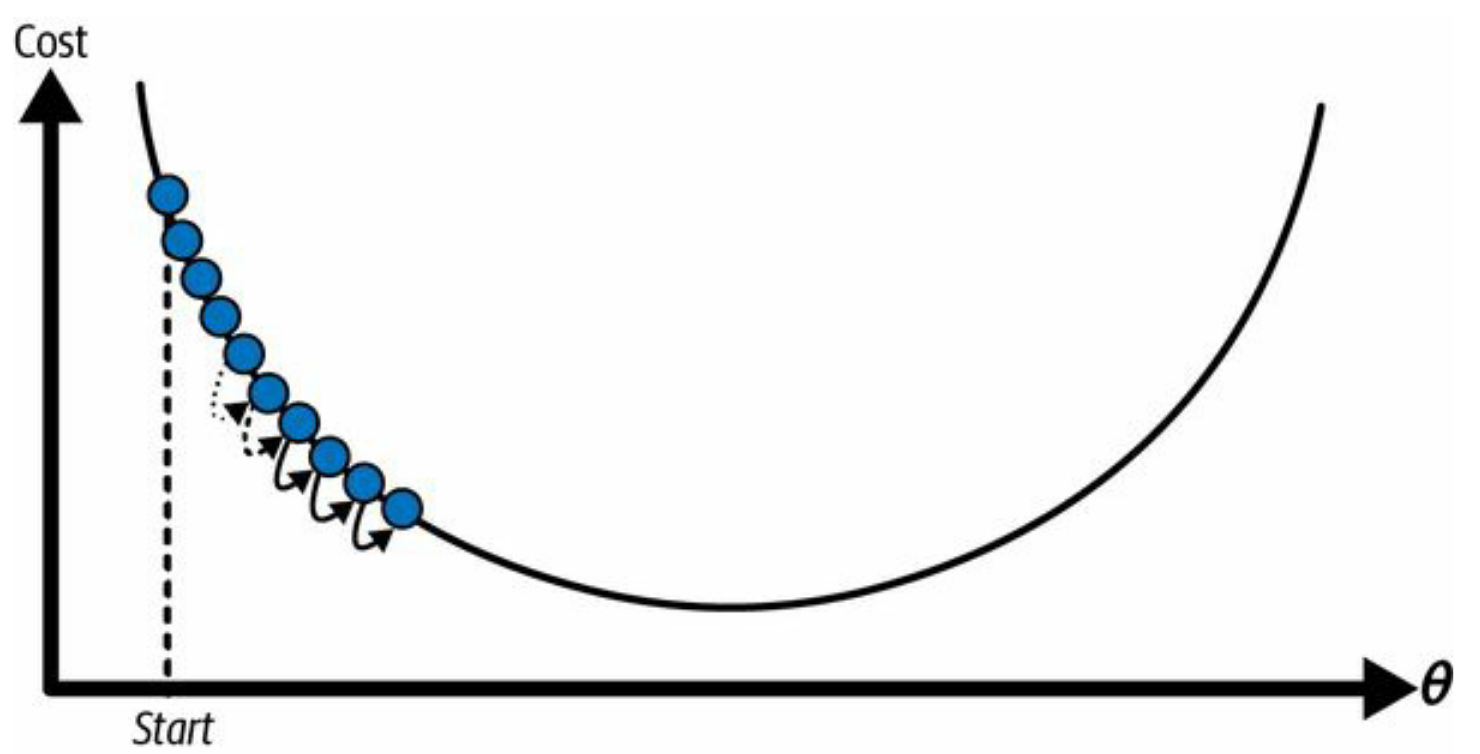
\includegraphics[width=0.5\linewidth, keepaspectratio]{img//chapter4/lr_small.png}\label{fig:lr_small}}
  \hfill
  \subfloat[]{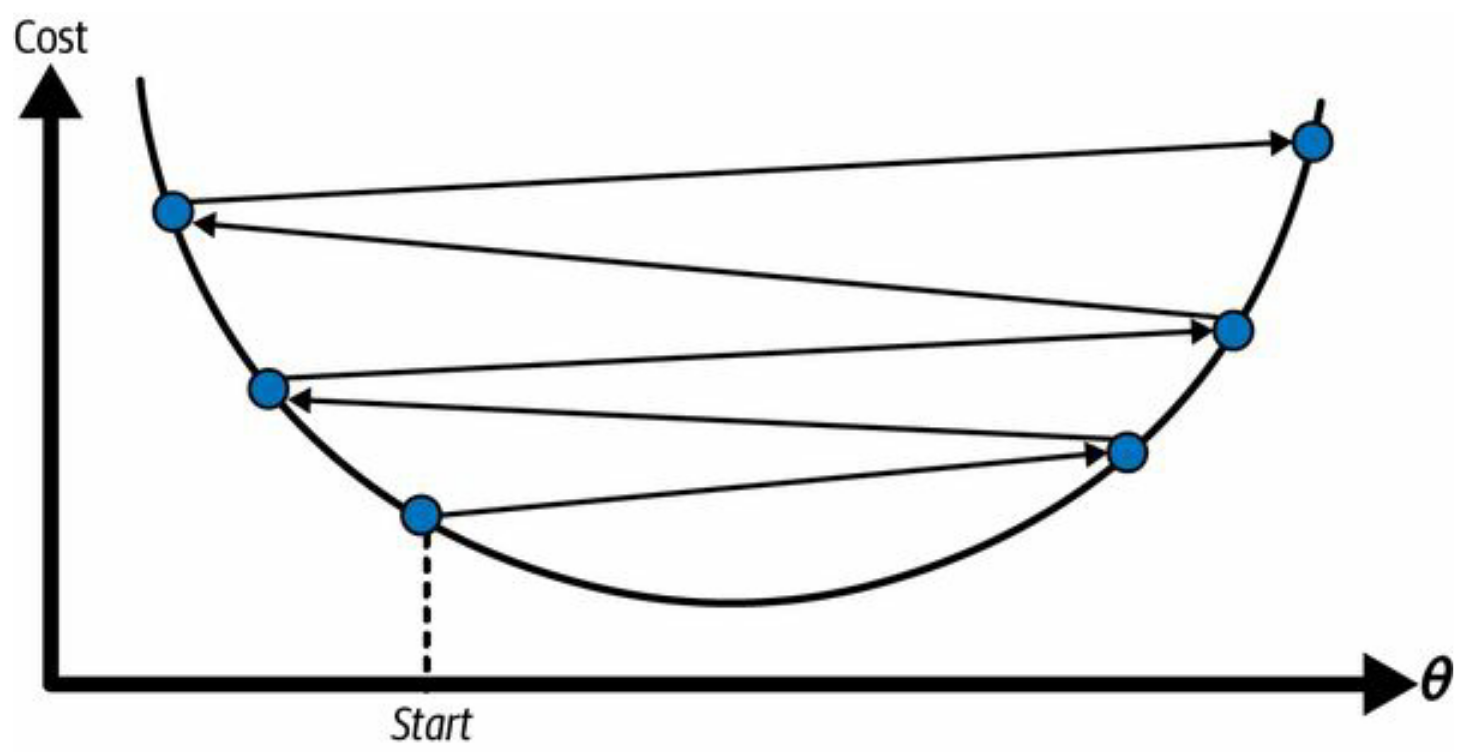
\includegraphics[width=0.5\linewidth, keepaspectratio]{img//chapter4/lr_high.png}\label{fig:lr_high}}
  \caption[Examples of learning rates too small or too high]{Examples of gradient descent for a one-dimensional loss (cost) function with \protect\subref{fig:lr_small} learning rate too small and \protect\subref{fig:lr_high} learning rate too high.\\\small{Credits: \cite{geron_hands-machine_2019}.}}
  \label{fig:lr_small_high}
\end{figure}
\newpage
All gradient-based optimization logic is encapsulated in the \emph{optimizer} object: it determines the direction in which the model parameters should be adjusted and the magnitude of the parameter update (learning rate).

Advanced optimizers, such as Adam \citep{kingma_adam_2017} and AdaDelta \citep{zeiler_adadelta_2012}, go beyond the basic gradient descent by adapting the learning rate during the training process based on the properties of the loss surface (\eg, its curvature). These optimizers can accelerate convergence by dynamically adjusting the step size for each parameter individually, based on the history of gradients. This can be particularly beneficial for navigating complex loss surfaces with varying curvatures.


%%%%%%%%%%%%%%%%%%%%%%%%%%%%%%%%%%%%%%%%%%%%%%%%%%%%%%%
%%%%% SubSubSec: Training loop %%%%%
%%%%%%%%%%%%%%%%%%%%%%%%%%%%%%%%%%%%%%%%%%%%%%%%%%%%%%%
\subsubsection{Training loop}
\label{subsubsec:training_loop}
Having outlined all the essential components within the optimization framework, it is now possible to describe the training process in all its phases, as shown in \cref{fig:backpropagation_algorithm}.
\begin{enumerate}
    \item \textbf{Initialization}: set up the model to be optimized and initialize its parameters to some (random) values.
    \item \textbf{Forward pass}: obtain the model predictions based on the initial parameters and compute the loss to quantify how far the model's outputs are from the actual target/observed values.
    \item \textbf{Backward pass (backpropagation)}: calculate the gradient of the loss function with respect to each parameter in the model. This involves propagating the error backwards from the outputs to the inputs, as described in \cref{subsubsec:reverse_mode}. This process systematically computes the partial derivatives using the chain rule to effectively determine how each parameter should be adjusted to minimize loss.
    \item \textbf{Parameter update (gradient descent)}: for each parameter, update its value by moving it in the direction that minimally decreases the loss
    \be
    \label{eq:4.12}
    \va{\t}_{final} = \va{\t}_{initial} - \eta \va{\nabla}_{\va{\t}_{initial}} f(\va{\t}_{initial}) \,.
    \ee
    \item \textbf{Iteration or convergence}: repeat steps 2 through 4 for a predefined number of iterations (or \emph{epochs}) or until the change in the loss function between iterations falls below a small threshold, indicating convergence.
\end{enumerate}

\begin{figure}
    \centering
    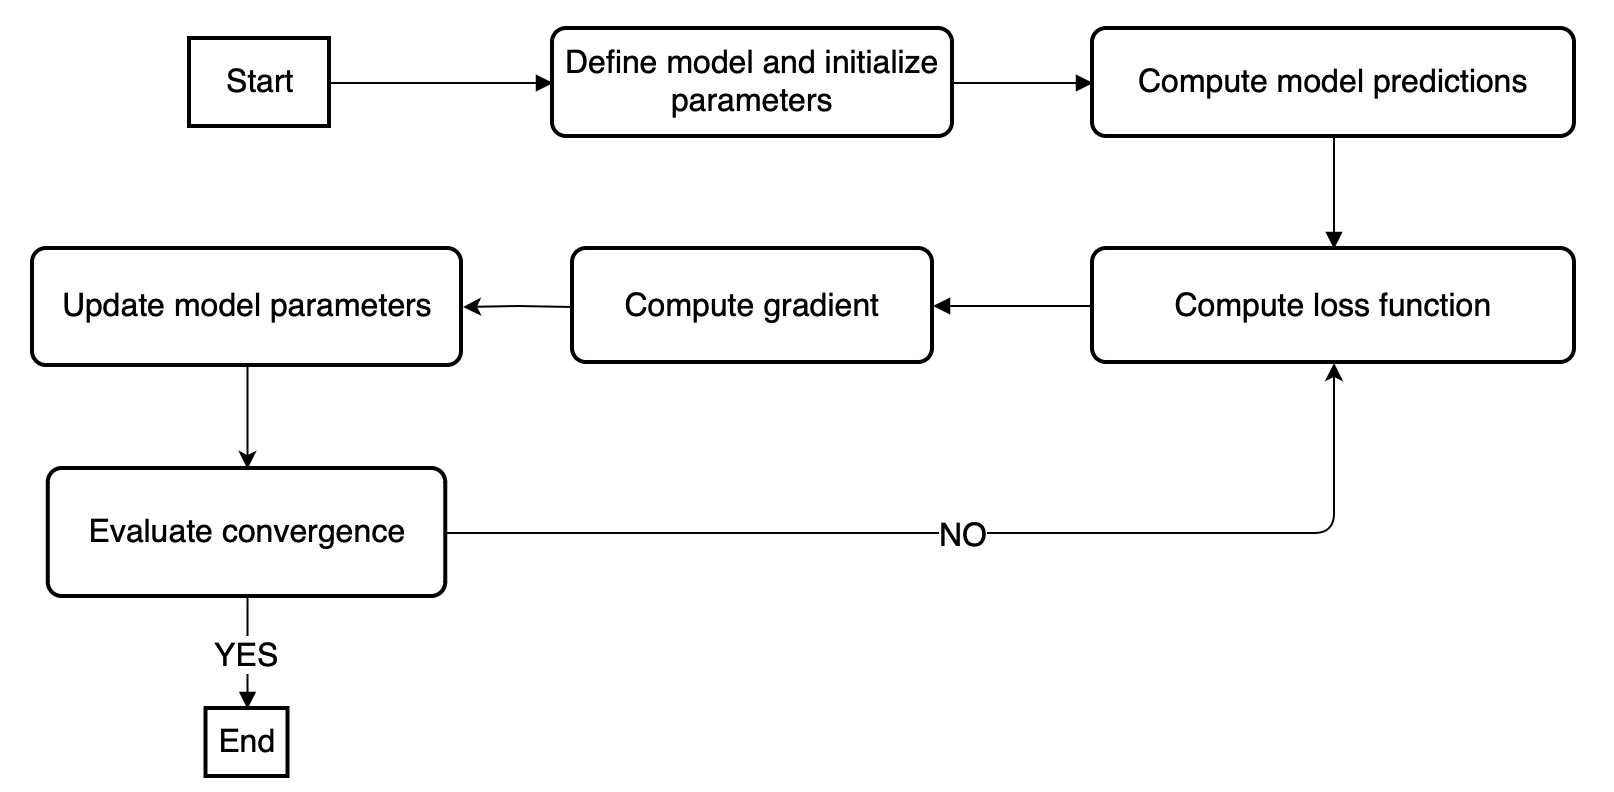
\includegraphics[width=\linewidth, keepaspectratio]{img//chapter4/backpropagation.png}
    \caption[Optimization algorithm diagram]{Optimization algorithm diagram.}
    \label{fig:backpropagation_algorithm}
\end{figure}